\section{Phase Extraction}
\label{sec:phase-extraction-problem}

In this section we define a new problem, which we call \emph{phase extraction}. In some sense, this problem can be seen as the inverse of the simulation problem: while, in order to simulate an Hamiltonian, we need to construct the complex exponential of the given matrix, in the phase extraction problem we essentially want to extract its complex logarithm.

\begin{problem}[Phase Extraction]
    \label{def:phase-extraction}
    Let $H$ be an Hermitian matrix satisfying $||H|| < 1$. Given a controlled version of the unitaries $U = e^{i \pi H}$ and $U^\dag = e^{-i \pi H}$ as oracles and $\varepsilon > 0$, construct a quantum circuit $C_U$ such that:
    $$||\bra{0}_A C_U \ket{0}_A - H|| \le \varepsilon,$$
    where $A$ is the subsystem containing ancilla registers.
\end{problem}
\noindent In other words, if we initially have a quantum circuit acting on its eigenbasis $\{ \ket{\phi_k} \}_k$ as
\begin{align*}
    U \ket{\phi_k} = e^{i \pi \varphi_k} \ket{\phi_k}
\end{align*}
for $\varphi_k \in [0, 1)$, we would like $C_U$ to act on the same eigenbasis as
\begin{align*}
    C_U \ket{0} \ket{\phi_k} = \varphi_k \ket{0} \ket{\phi_k} + \ket{1} \ldots \ .
\end{align*}
Thus, $C_U$ will contain a so-called \emph{block encoding} of the matrix $H$. The reader might argue that the stated problem is ill-defined: a global phase on $U$ would change our desired output, but not the input. However, it is important to note that the unitaries $U, U^\dag$ have to be given in their \emph{controlled} versions, where a global phase on $U$ would be seen as a controlled phase kickback. Moreover, it is worth remarking that this problem is substantially different from the well-known \emph{phase-estimation} problem, where one wants to achieve classical information about~$\varphi_k$, given $\ket{\phi_k}$.

Now we would like to use the quantum eigenvalue transform to apply a polynomial transformation of the eigenvalues of $U$, using the oracles we have. In particular, Haah's work tells us that any Laurent polynomial transformation $F: U(1) \rightarrow SU(2)$ of degree $n$ can be implemented using the QSP construction with only $\bigO(n)$ calls to $U, U^\dag$, provided that $F$ has definite parity (see Appendix~\ref{apx:haah-construction}). It is sufficient for us to have a desired transformation $f: U(1) \rightarrow [-1, 1]$ on one entry of this matrix (from now on we will assume without loss of generality that this entry is the top-left one, i.e., $f(z) = \bra{0} F(z) \ket{0}$).

Therefore, all we need now is to design a class of polynomials uniformly approximating a function of the phase. An interesting observation is that Laurent polynomials on the unit circle can be constructed using Fourier series.

\begin{observation}
    \label{thm:phase-extraction-poly}
    Let $\phi : \R \mapsto \R$ be a $2\pi$-periodic function whose Fourier series uniformly converges, and let $f : U(1) \mapsto \R$ be such that, for any real $x$,
    \begin{align*}
        f(e^{i x}) = \phi(x)
    \end{align*}
    holds. Then, there is a sequence of complex (Laurent) polynomials $P_n : \C \mapsto \C$ which uniformly converges to $f$ on the unit circle.
\end{observation}
This theorem tells us that we can construct a sequence of Laurent polynomials approximating any function of the eigenphase, and this will inherit all the strong convergence properties of Fourier sequences in our domain of interest. From now on, we use $\bar{\phi}(z)$ to denote the Laurent polynomial (or Laurent series) that satisfies $\bar{\phi}(e^{ix}) = \phi(x)$ for any real $x$. Notice that such function is unique since polynomials are fully defined by their behaviour on an infinite set.
\begin{proof}
    If $\phi(x) = \sum_{k \in \Z} c_k e^{i k x}$ is the Fourier series of $\phi(x)$, then
    \begin{align*}
        \bar{\phi}(z) = \sum_{k \in \Z} c_k z^k
    \end{align*}
    and this function is equal to $f$ on the unit circle. If $P_n(x) = \sum_{k = -n}^n c_k e^{ikx}$, then it is sufficient to see:
    \begin{align*}
        ||P_n - \phi||_{\R} = ||\bar{P}_n - \bar{\phi}||_{U(1)} = ||\bar{P}_n - f||_{U(1)},
    \end{align*}
    and the first norm tends to zero as $n \rightarrow \infty$.
\end{proof}
This result can be used to solve an extension of Problem~\ref{def:phase-extraction}. Indeed, we can compute a block encoding of $\phi(H)$ for an arbitrary real function $\phi$, provided it is sufficiently `well-behaved'.

Let us solve Problem~\ref{def:phase-extraction} using this technique: we would like that, for $\theta \in (-\pi, \pi]$, the eigenvalue $e^{i \theta}$ is mapped to $\theta/\pi$. Realistically, we cannot approximate this function in the whole interval, since there is a discontinuity in $\theta = \pm \pi$ and, because of this, the Fourier sequence could take too long to converge, or it could not uniformly converge at all. Therefore, we give up a small portion of the interval: for some small $\delta > 0$, we design a function $\phi_\delta(x)$ that is equal to $\phi(x) = x/\pi$ for every $x \in (-\pi + \delta, \pi - \delta)$, while in the neighbourhoods of $\pm \pi$ we replace its derivative with something continuous and piecewise linear that preserves the $2\pi$-periodicity of $\phi_\delta(x)$ (see Figure~\ref{fig:function-approx}). This implies that $\phi_\delta \in C^1$ by construction and, intuitively, the associated Fourier sum will converge faster. As a consequence, we will have to restrict Problem~\ref{def:phase-extraction} to instances with $||H|| \le 1 - \delta$.

\begin{figure}
    \centering
    \begin{subfigure}[b]{\columnwidth}
         \centering
         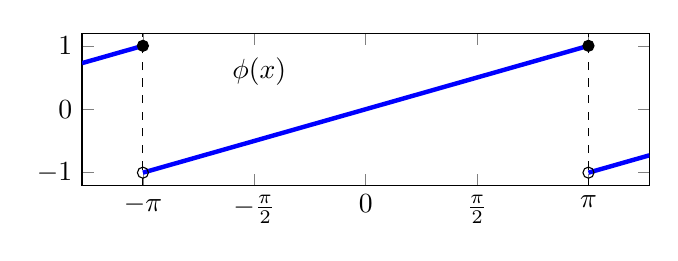
\begin{tikzpicture}
\begin{axis}[
    width=250pt,height=100pt,
    xmin=-4,xmax=4,
    ymin=-1.2,ymax=1.2,
    samples=50,
    xtick={-pi, -pi/2, 0, pi/2, pi},
    xticklabels={$-\pi$, $-\frac{\pi}{2}$, $0$, $\frac{\pi}{2}$, $\pi$},
    grid style={line width=.1pt, draw=gray!10},
    axis line style={latex-latex}]
    
    \addplot[blue, ultra thick, domain=-pi:pi] (x, x/pi);
    \addplot[blue, ultra thick, domain=-4:-pi] (x, x/pi + 2);
    \addplot[blue, ultra thick, domain=pi:4] (x, x/pi - 2);

    \addplot[mark=*] coordinates {(-pi,1)};
    \addplot[mark=o] coordinates {(-pi,-1)};
    \addplot[mark=*] coordinates {(pi,1)};
    \addplot[mark=o] coordinates {(pi,-1)};

    \draw [dashed] (axis cs:{-pi},-2) -- (axis cs:{-pi},2);
    \draw [dashed] (axis cs:{pi},-2) -- (axis cs:{pi},2);

    \node at (axis cs:-1.5,0.6) {$\phi(x)$};
  
\end{axis}
\end{tikzpicture}
    \end{subfigure}
    \hfill
    \begin{subfigure}[b]{\columnwidth}
        \centering
        \def\dlt{0.4}
\begin{tikzpicture}
\begin{axis}[
    width=250pt,height=110pt,
    xmin=-4,xmax=4,
    ymin=-1.2,ymax=1.45,
    samples=50,
    xtick={-pi, -pi/2, 0, pi/2, pi},
    xticklabels={$-\pi$, $-\frac{\pi}{2}$, $0$, $\frac{\pi}{2}$, $\pi$},
    grid style={line width=.1pt, draw=gray!10}]
    
    \addplot[red, ultra thick, domain=-pi+\dlt:pi-\dlt] (x, x/pi);
    \addplot[red, ultra thick, domain=-4:-pi-\dlt] (x, x/pi + 2);
    \addplot[red, ultra thick, domain=pi+\dlt:4] (x, x/pi - 2);

    \addplot[red, ultra thick, domain=-pi:-pi+\dlt] (x, x/pi + x*x/\dlt/\dlt + 2*pi*x/\dlt/\dlt - 2*x/\dlt + 1 + pi*pi/\dlt/\dlt - 2*pi/\dlt);
    \addplot[red, ultra thick, domain=-pi-\dlt:-pi] (x, 1 - 2*pi/\dlt - 2*x/\dlt + x/pi - pi*pi/\dlt/\dlt - pi*x/\dlt/\dlt - pi*x/\dlt/\dlt - x*x/\dlt/\dlt);
    \addplot[red, ultra thick, domain=pi-\dlt:pi] (x, -1 + 2*pi/\dlt - 2*x/\dlt + x/pi - pi*pi/\dlt/\dlt + pi*x/\dlt/\dlt + pi*x/\dlt/\dlt - x*x/\dlt/\dlt);
    \addplot[red, ultra thick, domain=pi:pi+\dlt] (x, -1 + 2*pi/\dlt - 2*x/\dlt + x/pi + pi*pi/\dlt/\dlt - pi*x/\dlt/\dlt - pi*x/\dlt/\dlt + x*x/\dlt/\dlt);

    \draw [dashed] (axis cs:{pi-\dlt},-2) -- (axis cs:{pi-\dlt},2);
    \draw [dashed] (axis cs:{pi+\dlt},-2) -- (axis cs:{pi+\dlt},2);
    \draw [dashed] (axis cs:{-pi-\dlt},-2) -- (axis cs:{-pi-\dlt},2);
    \draw [dashed] (axis cs:{-pi+\dlt},-2) -- (axis cs:{-pi+\dlt},2);

    \draw[|<->|] (axis cs:{-pi-\dlt},1) -- node[above] {$2\delta$} (axis cs:{-pi+\dlt},1);
    \draw[|<->|] (axis cs:{pi-\dlt},1) -- node[above] {$2\delta$} (axis cs:{pi+\dlt},1);

    \node at (axis cs:-1.5,0.85) {$\phi_\delta(x)$};
    
\end{axis}
\end{tikzpicture}
\undef\dlt
    \end{subfigure}
    \caption{Construction of $\phi_\delta(x)$ from $\phi(x)$. The two functions are identical except in the $\delta$-neighbourhood of the odd multiples of $\pi$. We have that $\phi_\delta \in C^1$ for any $\delta > 0$, so its Fourier series will converge faster than the series of $\phi(x)$.}
    \label{fig:function-approx}
\end{figure}

\begin{theorem}
    \label{thm:phase-extraction-jackson-rate}
    The function $\bar{\phi}_\delta : U(1) \rightarrow \R$ defined as
    \begin{align*}
        \bar{\phi}_\delta(e^{ix}) = \phi_\delta(x)
    \end{align*}
    for every $x \in \R$ can be $\epsilon$-approximated on the unit circle using a polynomial of degree
    $$d = \Tilde{\bigO}\left(\frac{1}{\delta} \sqrt{\frac{1}{\epsilon}}\right).$$
\end{theorem}
\begin{proof}
    Let $S_{\delta, d}(x) = \sum_{k = -d}^{d} c_k e^{ikx}$ be the Fourier sum of $\phi_\delta$ up to terms of degree $d$. By a result of Jackson~\cite[pp.\ 20--25]{jacksonTheoryApproximation1930a} we know that, since $\phi_\delta \in C^1$ and $\phi'_\delta$ is $2/\delta^2$-Lipschitz, the approximation error of the $d$-th degree Fourier sum is bounded by
    \begin{align*}
        ||S_{\delta, d} - \phi_\delta||_{\R} \le K \frac{\log d}{\delta^2 d^2} = K \frac{1}{\delta^2 d^{2-o(1)}}
    \end{align*}
    for some absolute constant $K$. The above is bounded by $\epsilon$ when $d^{2-o(1)} = \bigO\left(\frac{1}{\epsilon \delta^2}\right)$ or, in other words
    \begin{align*}
        d = \Tilde{\bigO}\left( \frac{1}{\delta} \sqrt{\frac{1}{\epsilon}} \right).
    \end{align*}
    This concludes the proof since we can replace $e^{ix} = z$ in $S_{\delta, d}$ to obtain the sequence of Laurent polynomials $\bar{S}_{\delta, d}$ uniformly converging to $\bar{\phi}_\delta$ on the unit circle with the same rate.
\end{proof}
It is interesting to point out that, if one only cares about a constant $\delta$ (e.g., $\delta = \pi/2$ so we get our good approximation only on the right semicircle), one could increase the smoothness of $\phi_\delta$ to get a better dependence from $1/\epsilon$. The Lipschitz constant increases, but it would only depend on $\delta$. We investigate this improvement in Section~\ref{sec:inductive-smoothening}.

Now we have a Laurent polynomial approximating the function $\bar{\phi}_\delta$ that we would like to achieve. We need to take care of one last problem: remember that Haah's construction requires the Laurent polynomial to be either even or odd. Keep in mind that $\bar{\phi}_\delta(z)$ does not have definite parity (and so do not its approximating polynomials), even though $\phi_\delta$ is odd.

A simple workaround is to split $\bar{S}_{\delta, d}(z)$ into even and odd polynomials $\bar{S}^0_{\delta, d}(z), \bar{S}^1_{\delta, d}(z)$, implement them separately, and then add them up using a simple block encoding (see Figure~\ref{fig:block-encoding-sum-circuit}). The phase extraction function $\phi(x)$ can be split into $\phi_0, \phi_1$ such that $\phi_0(x) = \phi_0(x + \pi)$ and $\phi_1(x) = -\phi_1(x + \pi)$ (the reader can check that the Laurent polynomials associated to their Fourier series are even and odd, respectively). Moreover, both of them are bounded by~$1/2$ in absolute value everywhere, and the sum of their Laurent polynomials gives exactly the Laurent polynomial of $\phi$ (see Figure~\ref{fig:function-approx-even-odd}).

\begin{figure}
    \centering
    \begin{subfigure}[b]{\columnwidth}
         \centering
         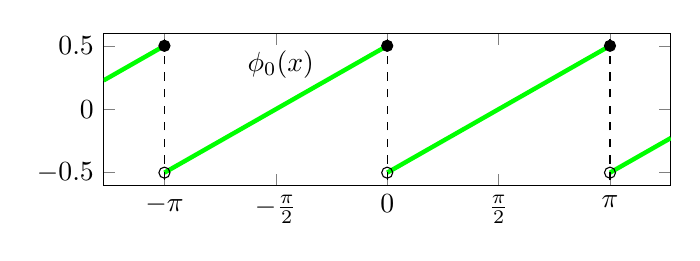
\begin{tikzpicture}
\begin{axis}[
    width=250pt,height=100pt,
    xmin=-4,xmax=4,
    ymin=-0.6,ymax=0.6,
    samples=50,
    xtick={-pi, -pi/2, 0, pi/2, pi},
    xticklabels={$-\pi$, $-\frac{\pi}{2}$, $0$, $\frac{\pi}{2}$, $\pi$},
    grid style={line width=.1pt, draw=gray!10},
    axis line style={latex-latex}]
    
    \addplot[green, ultra thick, domain=-pi:0] (x, x/pi + 1/2);
    \addplot[green, ultra thick, domain=0:pi] (x, x/pi - 1/2);
    \addplot[green, ultra thick, domain=pi:4] (x, x/pi - 3/2);
    \addplot[green, ultra thick, domain=-4:-pi] (x, x/pi + 3/2);

    \addplot[mark=*] coordinates {(-pi,1/2)};
    \addplot[mark=o] coordinates {(-pi,-1/2)};
    \addplot[mark=*] coordinates {(0,1/2)};
    \addplot[mark=o] coordinates {(0,-1/2)};
    \addplot[mark=*] coordinates {(pi,1/2)};
    \addplot[mark=o] coordinates {(pi,-1/2)};

    \draw [dashed] (axis cs:{-pi},-2) -- (axis cs:{-pi},2);
    \draw [dashed] (axis cs:0,-2) -- (axis cs:0,2);
    \draw [dashed] (axis cs:{pi},-2) -- (axis cs:{pi},2);

    \node at (axis cs:-1.5,0.35) {$\phi_0(x)$};
  
\end{axis}
\end{tikzpicture}
    \end{subfigure}
    \hfill
    \begin{subfigure}[b]{\columnwidth}
        \centering
        \input{figures/function-approx-odd.tex}
    \end{subfigure}
    \caption{Plots of $\phi^0(x)$ and $\phi^1(x)$. One can see that their sum will give exactly $\phi(x)$. Since $\phi(x + \pi) = \bar{\phi}(e^{i(x + \pi)}) = \bar{\phi}(-e^{ix})$, this determines the parity of the approximating Laurent polynomials.}
    \label{fig:function-approx-even-odd}
\end{figure}

In the end, this procedure has a certain failure probability due to non-unitarity of the matrix we are extracting, which can be mitigated by classical repetition or amplitude amplification techniques~\cite{brassardQuantumAmplitudeAmplification2002, berryExponentialImprovementPrecision2014a, berrySimulatingHamiltonianDynamics2015}. It is now important to estimate the initial probability of measuring $\ket{00}$ (i.e., our success probability), in order to bound the multiplicative factor that the amplifying procedure gives to our overall complexity. However, this strictly depends on the unitary $U$ whose phases we want to extract: for example, if $U$ has all the eigenphases close to $0$, then all of them will be mapped to very small amplitudes by $\bar{\phi}_\delta(z)$, giving us a low probability of success, which is harder to amplify. In the next section we will see a concrete example.

\begin{figure}
    \centering
    \begin{quantikz}
    \lstick{$\ket 0_A$} & \gate{H} & \octrl{1} & \ctrl{1} & \gate{H} & \qw \\
    \lstick{$\ket 0_B$} & \qw & \gate[wires=2]{
    \begin{bmatrix}
        \bar S^0(U) & \cdot \\
        \cdot & \cdot
    \end{bmatrix}
    } & \gate[wires=2]{
    \begin{bmatrix}
        \bar S^1(U) & \cdot \\
        \cdot & \cdot
    \end{bmatrix}
    } & \qw & \qw \\
    \lstick{$\ket\phi$} & \qw & & & \qw & \qw
\end{quantikz}
    \caption{Implementation of the block encoding for summing two matrices. The two big gates represent a quantum eigenvalue transform on the unitary $U$ implementing the polynomials $\bar S^0, \bar S^1$. If $\ket{00}$ is measured on the two control qubits, then $\ket{\phi}$ will be transformed by the matrix $\bar S^0(U) + \bar S^1(U) \equiv \bar S(U)$, implementing the original Fourier approximation.}
    \label{fig:block-encoding-sum-circuit}
\end{figure}